%TC第29.1节练习 4、5
%TC第29.2节练习 2、4、6
%TC第29.3节练习 5
%TC第29.4节练习 2
%%%%%%%%%%%%%%%%%%%%%%%%%%%%%%%%%%%%%%%%%%%%%%%%%%%%%%%%%%%%%%%%
\documentclass[11pt, a4paper, UTF8]{ctexart}
%%%%%%%%%%%%%%%%%%%%%%%%%%%%%%%%%%%
% File: preamble.tex
%%%%%%%%%%%%%%%%%%%%%%%%%%%%%%%%%%%

\usepackage[top = 1.5cm]{geometry}

% Set fonts commands
\newcommand{\song}{\CJKfamily{song}} 
\newcommand{\hei}{\CJKfamily{hei}} 
\newcommand{\kai}{\CJKfamily{kai}} 
\newcommand{\fs}{\CJKfamily{fs}}

\newcommand{\me}[2]{\author{{\bfseries 姓名:}\underline{#1}\hspace{2em}{\bfseries 学号:}\underline{#2}}}

% Always keep this.
\newcommand{\noplagiarism}{
  \begin{center}
    \fbox{\begin{tabular}{@{}c@{}}
      请独立完成作业,不得抄袭。\\
      若得到他人帮助, 请致谢。\\
      若参考了其它资料,请给出引用。\\
      鼓励讨论,但需独立书写解题过程。
    \end{tabular}}
  \end{center}
}

% Each hw consists of three parts:
% (1) this homework
\newcommand{\beginthishw}{\part{作业}}
% (2) corrections (Optional)
\newcommand{\begincorrection}{\part{订正}}
% (3) any feedback (Optional)
\newcommand{\beginfb}{\part{反馈}}

% For math
\usepackage{amsmath}
\usepackage{amsfonts}
\usepackage{amssymb}

% Define theorem-like environments
\usepackage[amsmath, thmmarks]{ntheorem}

\theoremstyle{break}
\theorembodyfont{\song}
\theoremseparator{}
\newtheorem*{problem}{题目}


\theoremheaderfont{\kai\bfseries}
\theoremseparator{:}
% \newtheorem*{remark}{注}
\theorempostwork{\bigskip\hrule}
\newtheorem*{solution}{解答}
\theorempostwork{\bigskip\hrule}
\newtheorem*{revision}{订正}

\theoremstyle{plain}
\newtheorem*{cause}{错因分析}
\newtheorem*{remark}{注}

\theoremstyle{break}
\theorempostwork{\bigskip\hrule}
\theoremsymbol{\ensuremath{\Box}}
\newtheorem*{proof}{证明}

\renewcommand\figurename{图}
\renewcommand\tablename{表}

% For figures
% for fig with caption: #1: width/size; #2: fig file; #3: fig caption
\newcommand{\fig}[3]{
  \begin{figure}[htp]
    \centering
      \includegraphics[#1]{#2}
      \caption{#3}
  \end{figure}
}

% for fig without caption: #1: width/size; #2: fig file
\newcommand{\fignocaption}[2]{
  \begin{figure}[htp]
    \centering
    \includegraphics[#1]{#2}
  \end{figure}
}
\usepackage{blindtext}
\usepackage[utf8]{inputenc}
\usepackage{amsmath,bm}
\usepackage{amstext}
\usepackage{amsfonts}
\usepackage{amsmath}
\usepackage[colorlinks,linkcolor=blue]{hyperref}
\title{机器学习导论}
\me{殷天润}{171240565}
\date{\today}

\begin{document}
\maketitle
\noplagiarism

%%%%%%%%%%%%%%%%%%%%%%%%%%%%%%%%%%%%%%%%%%%%%%%%%%%%%%%%%%%%%%%%
%                       Homework START!                        %
%%%%%%%%%%%%%%%%%%%%%%%%%%%%%%%%%%%%%%%%%%%%%%%%%%%%%%%%%%%%%%%%
\beginthishw
%%%%%%%%%%%%%%%%%%%%
\begin{problem}[ML problem 1]
In multi-label problem, each instance $\bm{x}$ has a label set $\bm{y}=\{y_1,y_2,...,y_l\}$ and each label $y_i\in\{0,1\}$. Assume the post probability $p(\bm{y}|x)$ follows the conditional independence:\\
\begin{equation}
p(\bm{y}|x)=\prod\limits_{i=1}^l p(y_i|x).
\end{equation}
Please use the logistic regression method to handle the following questions.\\
(1) [15pts] Please give the 'log-likelihood' function of your logistic regression model;\\
(2) [10pts] Please calculate the gradient of your 'log-likelihood' function.\\     


\end{problem}
\begin{solution}
  \begin{enumerate}
  	\item %为了下面书写简约定义:$Y_1=(1,0,0,...0),Y_2=(0,1,0,....,0)...Y_l=(0,0,....1),Y_{l+1}=(0,0,.....0)$;$\theta ^{T}\bm{x}=w^{T}x+b$,$\bm{x}$是x扩了一列之后的项
  	
  	 
  	%softmax function:
  	%$$h(\bm{x})=\frac{1}{1+\sum _{i=1} ^{l} e^{\theta _{i}^{T}\bm{x}}}{
  %		\left[ \begin{array}{c}
 % 		e^{\theta _{1}^{T}\bm{x}} \\
 % 		e^{\theta _{2}^{T}\bm{x}}\\
  %		...\\
  %		e^{\theta _{l}^{T}\bm{x}} 
  %		\end{array}
  %		\right ]}$$
  %	
  %	其中: $p(Y_i|\bm{x})=\frac{e^{\theta_{i}^{T}\bm{x}}}{1+\sum _{i=1} ^{l} e^{\theta _{i}^{T}\bm{x}}}$
  %	
  %	因此对于给定数据集,$\{(x_i,y_i)\}_{i=1}^{m}$;对数似然函数('log-likelihood'):
  %	$$l(\bm{\theta})=\sum_{q=1}^{m}ln ~p(Y_i^{(q)}|\bm{x}^{(q)};\theta )=\sum_{i=1}^{m}ln \Pi^{k}_{t=1} (\frac{e^{\theta _{1}^{T}\bm{x}^{(q)}}}{1+\sum _{i=1} ^{l} e^{\theta _{i}^{T}\bm{x}^{(q)}}})$$
  
  根据$y_i$的组合,$Y_i=(y_1,.....y_n),y_i=\{0,1\}$有$2^{l}$次方种可能性;
  
  由于条件独立,对于每一种$Y_i$都有$p(Y_i)=\Pi_{j=1}^{l} p(y_{ij}|x)$;
  
  
  
  \begin{equation}
  \begin{aligned}
  &l(\bm{w}_1,\bm{w}_2,...\bm{w}_l;b_1,b_2,...,b_l)
  \\ &=\sum_{i=1}^{m}ln~p(Y_i|\bm{x};\bm{w_i},b_i)
  \\ &=\sum_{i=1}^{m} ln~(\Pi _{j=1}^{l} p(y_{ij}|x;\bm{w_i},b_i))
  \\ &=\sum_{i=1}^{m} \sum _{j=1}^{l} ln(p(y_{ij}|x;\bm{w_i},b_i))
  \end{aligned}
  \end{equation}

为了简化书写,增广$\bm{x}$,令$\hat{\bm{x}}=(\bm{x},1)$,$\bm{\beta}_{i}=(\bm {w}_i,b_i)$,此时可以简写$\bm{w}^{T}\bm{x}+b$为$\bm{\beta}_i^{T}\bm{x}$;

模仿西瓜书p59页的处理:令$p_{j1}(\hat{\bm{x}}_i;\bm{\beta}_i)=p(y_{ij}=1|\hat{\bm{x}};\bm{\beta}_i )$(表示第i组第j个y标签为1的概率),$p_{j0}(\hat{\bm{x}}_i;\bm{\beta}_i)=p(y_{ij}=0|\hat{\bm{x}};\bm{\beta}_i )=1-p(y_{ij}=1|\hat{\bm{x}};\bm{\beta}_i )$

因此可以重写极大似然项为:


$$p(y_{ij}|\bm{x}_i;\bm{w}_i,b_i)=y_ip_{j1}(\hat{\bm{x}}_i;\bm{\beta}_i);\bm{\beta}_i )+(1-y_i)p_{j0}(\hat{\bm{x}}_i;\bm{\beta}_i)$$

将这个式子带入到公式(2)中,将最大化(2)式转化成最下化下式有:
$$l(\bm{\beta_{1}},\bm{\beta_{2}},\bm{\beta_{3}}...,\bm{\beta_{l}})=\sum_{i=1}^{m} \sum _{j=1}^{l}(-y_{ij}\beta^{T}_j\hat{x_{i}}+ln(1+e^{\beta_{j}^{T}\hat{x}_i}))$$
  	\item 梯度计算:
  \begin{equation*}
  \begin{aligned}
  \nabla(l(\bm{\beta_{1}},\bm{\beta_{2}},\bm{\beta_{3}}...,\bm{\beta_{l}}))&=\frac{\partial l(\bm{\beta_{1}},\bm{\beta_{2}},\bm{\beta_{3}}...,\bm{\beta_{l}} )}{\partial(\bm{\beta_{1}},\bm{\beta_{2}},\bm{\beta_{3}}...,\bm{\beta_{l}})}\\&=-\sum_{i=1}^{m} \sum _{j=1}^{l}\hat{\bm{x}}_i(y_{ij}-p_{j1}(\hat{\bm{x}}_i;\bm{\beta} _{j}))
  \end{aligned}
  \end{equation*}
  	
  \end{enumerate}
    
\end{solution}




\begin{problem}[ML problem 2]
	
Suppose we transform the original $\bf X$ to $\hat{\bf Y}$ via linear regression . In detail, let 

\begin{equation*}
\hat{\bf Y} = \bf X(\bf X^{\top} \bf X)^{-1}\bf X^{\top}\bf Y = \bf X\hat{\bf B},
\end{equation*}
where $\bf X$ and $\bf Y$ are the feature and label matrix, respectively.
Similarly for any input $\mathbf{x}$, we get a transformed vector $\hat{\mathbf{y}} = \hat{\bf B}^{\top}\mathbf{x}$. Show that LDA using $\hat{\bf Y}$ is identical to LDA in the original space.

\end{problem}
\begin{solution}
	对于给定的数据集D=$\{(x_i,y_i)\}_{i=1}^{m},y_i=\{0,1\}$,定义class数量是K
  \begin{enumerate}
  	\item 首先讨论X的平均值,便于后面替换:$$\mu=\frac{1}{m}\sum_{i=1}^{m}x$$
  	经过变换后:$$\hat{\mu}=\frac{1}{m}\sum_{i=1}^{m}\hat{y}=\frac{1}{m}\hat{B}^{T}\sum_{i=1}^{m}x=\hat{B}^{T}\mu$$
  	\item 现在讨论类内散度矩阵(within-class scatter matrix)和类间散度矩阵(scatter matrix)
  	$$S_w=\sum _{i=1}^{K} \sum _{x\in X_i}(x-\mu _i)(x-\mu _i)^{T}$$
  	$$\hat{S_w}=\sum _{i=1}^{K} \sum _{x\in X_i}(\hat{B}^{T}x-\hat{B}^{T}\mu _i)(\hat{B}^{T}x-\hat{B}^{T}\mu _i)^{T}=\hat{B}^{T}\sum _{i=1}^{K} \sum _{x\in X_i}(x-\mu _i)(x-\hat\mu _i)^{T}\hat{B}=\hat{B}^{T}S_w\hat{B}$$
  	同理,$$\hat{S_b}=\hat{B}^{T}S_b\hat{B}$$
  	\item 因此 现在考虑J(w)
  	$$J(w)=\frac{w^TS_bw}{w^TS_ww}$$
  	$$\hat{J(w)}=\frac{w^T\hat{S_b}w}{w^T\hat{S_w}w}=\frac{w^T\hat{B}^TS_b\hat{B}w}{w^T\hat{B}^TS_w\hat{B}w}=\frac{(\hat{B}w)^TS_b(\hat{B}w)}{(\hat{B}w)^TS_w(\hat{B}w)}$$
  	
  	令w'=$\hat{B}w$,可见LDA using $\hat{\bf Y}$ is identical to LDA in the original space.
  \end{enumerate}
\end{solution}

\begin{problem}[ML problem 3]
\end{problem}
\subsection{[55pts] Logistic Regression from scratch  }
Implementing algorithms is a good way of understanding how they work in-depth. In case that you are not familiar with the pipeline of building a machine learning model, this article can be an example (\href{https://www.jianshu.com/p/ecb89148ed64}{here}).

In this experiment, you are asked to build a classification model on one of UCI data sets, Letter Recognition Data Set
(\href{http://lamda.nju.edu.cn/ml2019/ML2019-PS2-dataset.zip}{click to download}). In particular, the objective is to identify each of a large number of black-and-white
rectangular pixel displays as one of the 26 capital letters in the English alphabet. The detailed statistics of this data set is listed in Table~\ref{tab:dataset}. The data set was then randomly split into train set and test set with proportion $7:3$. Also, letters from `A' to `Z' are mapped to digits `1' to `26' respectively as represented in the last column of the provided data set.


\begin{table}[!ht]
	\centering
	\caption{Statistics of the data set.}
	\vspace{2mm}
	\label{tab:dataset}
	\begin{tabular}{|c|c|c|}
		\hline
		Property & Value & Description\\
		\hline
		Number of Instances & 20,000 & Rows of the data set\\
		\hline
		Number of Features & 17 & Columns of the data set\\
		\hline
		Number of classes & 26 & Dimension of the target attribute \\
		\hline
	\end{tabular}
\end{table}


In order to build machine learning models, you are supposed to implement Logistic Regression (LR) algorithm which is commonly used in classification tasks. Specifically, in this experiment, you have to adapt the traditional binary class LR method to tackle the multi-class learning problem. 

\begin{enumerate}
	\item[(1)] [\textbf{5pts}] You are encouraged to implement the code using \emph{Python3} or \emph{Matlab}, implementations in any other programming language will not be judged. Please name the source file (which contains the main function) as \emph{LR\underline{\hspace{0.5em}}main.py} (for python3) or \emph{LR\underline{\hspace{0.5em}}main.m} (for matlab). Finally, your code needs to print the testing performance on the provided test set once executed.
	
	\item[(2)] [\textbf{30pts}] Functions required to implement:
	\begin{itemize}
		\item Implement LR algorithm using gradient descent or Newton's method.
		\item Incorporate One-vs-Rest (OvR) strategy to tackle multi-class classification problem.
	\end{itemize}
	\item[(3)] [\textbf{20pts}] Explain implementing details in your submitted report (source code should not be included in your report), including optimization details and hyper-parameter settings, etc. Also, testing performance with respect to Accuracy, Precision, Recall, and $F_1$ score should be reported following the form of Table 2.
\end{enumerate}

\begin{table}[h]
	\centering
	\caption{Performance of your implementation on test set.}
	\vspace{2mm}
	\label{tab:my_label}
	\begin{tabular}{|c|c|}
		\hline
		Performance Metric & Value (\%) \\
		\hline
		accuracy & 00.00 \\
		\hline
		micro Precision  & 00.00\\
		\hline
		micro Recall & 00.00\\
		\hline
		micro $F_1$ & 00.00\\
		\hline
		macro Precision  & 00.00\\
		\hline
		macro Recall & 00.00\\
		\hline
		macro $F_1$ & 00.00\\
		\hline
	\end{tabular}
	
\end{table}

\textbf{NOTE:} Any off-the-shelf implementations of LR or optimization methods are \textbf{NOT ALLOWED} to use. When submitting your code and report, all files should be placed in the same directory (without any sub-directory).

\begin{solution}
\begin{enumerate}
	\item 我已经独立写了python程序,名字是LR\_main.py;默认情况下:步长为0.09,迭代次数1000次,大约需要 分钟时间运行;运行前首先要确保环境是python3,需要有numpy,pandas以及csv包;
	\item 我使用了梯度下降法以及OVR来实现这个程序,梯度下降法实现了class LogisticClassfier,OVR思想实现了class OVRclassifier;我在之前尝试的时候还试过了随机梯度下降算法,但是效果不是很好,具体细节下面会说到;
	\item 这部分我将详细的描述我的实验,主要分为:程序模块介绍,程序优化过程,调参数据,实验结果这几个部分
	\begin{enumerate}
		\item 程序各个模块的介绍:
		我的程序主要包括:两个class:class LogisticClassfier,class OVRclassifier,四个def: def gradient,def sigmod\_fit\_matrix,def sigmod\_output\_matrix,def score组成;
		
		class LogisticClassfier:用梯度下降法实现的二分类器:
		
		\begin{enumerate}
			\item 训练的模块是def fit(self, X, Y),核心的部分是:
	
		
\includegraphics[scale=0.5]{1.png}\\
		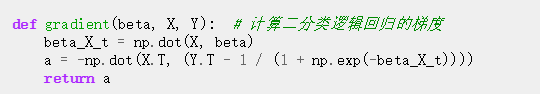
\includegraphics[scale=0.5]{2.png}\\
		
		\item 	预测的部分是def predict(self, X),用训练出来的beta通过sigmod函数进行预测
	
		\end{enumerate}
		
		class OVRclassifier:多分类器
		\begin{enumerate}
			\item def OVR\_train(self, X\_train, Y\_train):
			
			每一次选一个(chosen\_one)作为 "O",在Y\_train将对应的取值标为1,其余标为0,送给相应的二分类器list中的二分类器训练即可;
			
			\item def OVR\_predict(self, X\_test):
			
			运用相应的二分类器中的predict进行预测;
			
		\end{enumerate}
	\item 程序的优化过程:
	\begin{enumerate}
		\item 我主要对程序的速度进行了优化;
		
		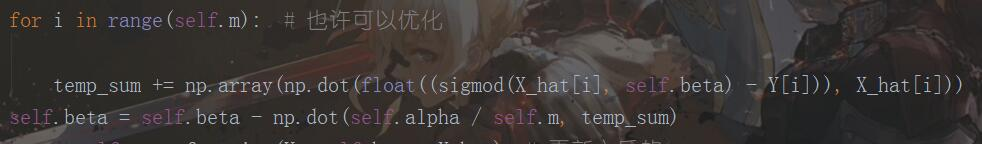
\includegraphics[scale=0.65]{o1.jpg}\\
		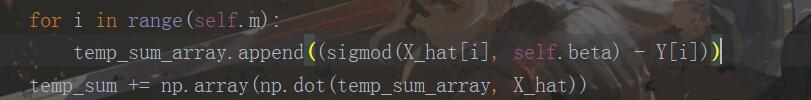
\includegraphics[scale=0.65]{o2.jpg}\\
		
		上面是我之前两个版本的程序,第一个版本完全是按照西瓜书上的3.30式子写的,是一个for循环的矩阵运算;这个版本速度实在太慢;因此我修改成了下一个版本,减少了矩阵的运算,瓶颈变为了for循环下的sigmod函数运算,由于这个是对单个的元素进行运行,速度虽然是上个版本的感觉上的两倍,但是还是很慢,算一千次大概需要2-3个小时;因此我改成了目前这个版本,删去了for循环,将它化简为仅仅一个矩阵运算,速度快了很多,1000次的loop只需要5-10分钟!
		
		另外我选择了取平均值操作也就是除以m,这样对步长的要求更小而且每一次更新更加平稳;
		
		\item 除了仅仅依靠loop次数的退出方式,在调参的过程中我还根据书上的3.27式子,使用了辅助的cost\_function,可以依靠cost\_funtion的差值退出:
		
		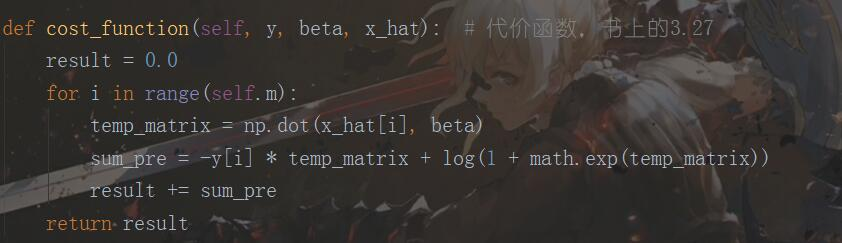
\includegraphics[scale=0.65]{cost.jpg}\\
		在运行梯度下降前我先跑一遍cost\_function,与运行后的值进行比较,就可以知道梯度下降对于beta拟合的贡献度,如果步长正常,前后两次的cost\_function的值应该差一个小的负数;如果出现
		
		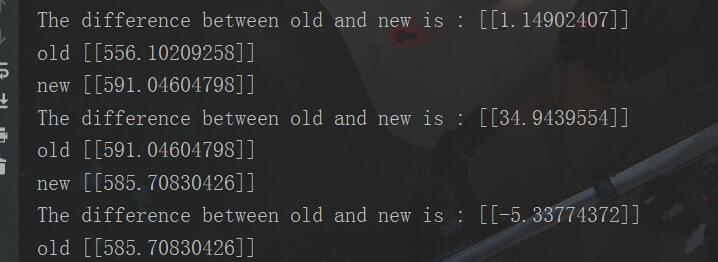
\includegraphics[scale=0.65]{in_test.jpg}\\
		
		这种情况,那么就可以一定意义上的判定自己的步长取的偏大,在不需要算出最后精确度的情况下就可以修改,一定意义上减少了调参时间;
		
		另外我在调参时也设计运行到loop的$\frac{9}{10}$之后就开始计算cost\_function的差值,并且设置accuracy,让差值小于这个accuracy之后就直接退出,避免过度拟合
	\end{enumerate}
	\item 调参:
	\begin{enumerate}
		\item 我额外做了随机梯度下降的尝试:
		
		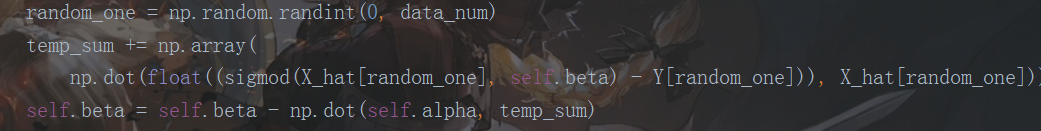
\includegraphics[scale=0.45]{random.png}\\
		但是效果并不好,当alpha取9.6e-07的时候,loop为500000的时候准确率为25.8\%,当alpha取0.0001的时候,loop为140000的时候准确率为13.25\%
		\item 我控制loop以及控制alpha做了相应的对比实验:
		
		可视化图表如下:
		\begin{enumerate}
			\item 固定alpha为0.09,改变loop次数;纵坐标的值表示accuracy,横坐标是loop次数:
			
			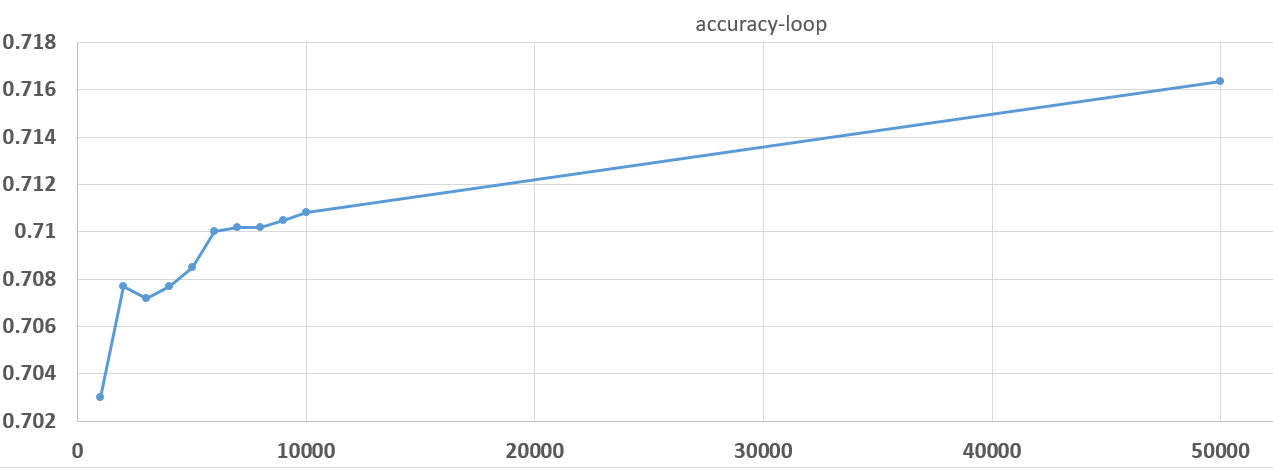
\includegraphics[scale=0.35]{accuracyandloop.png}\\
			
			\item 固定loop次数为10000,改变alpha;纵坐标的值表示accuracy,横坐标是alpha:
			
			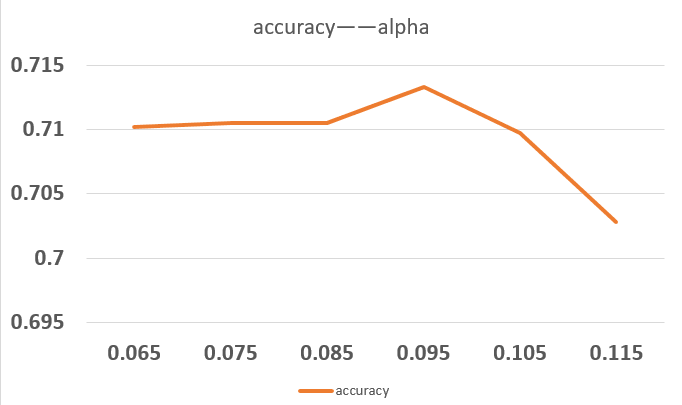
\includegraphics[scale=0.5]{accuracyandalpha.png}
		\end{enumerate}
	\end{enumerate}
	\item 实验结果:
	
	我选择下图作为我实验的结果,跑了十万次loop大概需要2-3个小时,如果复现请选择0.09,1000次这样的默认参数作为输入;
	
	\centering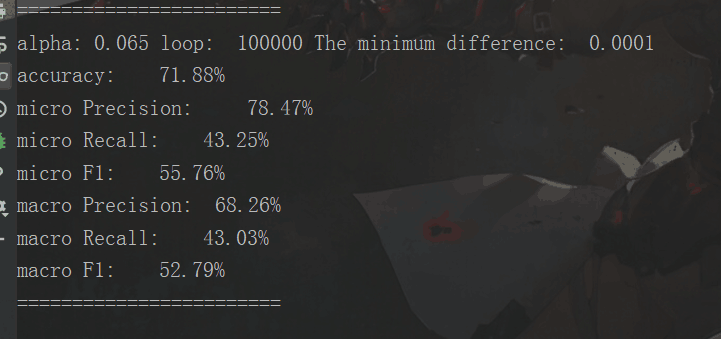
\includegraphics[scale=0.5]{result.png}\\
	
	
	
	\item \begin{table}[h]
		\centering
		\caption{Performance of my implementation on test set.}
		\vspace{2mm}
		\label{tab:my_label}
		\begin{tabular}{|c|c|}
			\hline
			Performance Metric & Value (\%) \\
			\hline
			accuracy &71.88 \\
			\hline
			micro Precision  & 78.47\\
			\hline
			micro Recall & 43.25\\
			\hline
			micro $F_1$ & 55.76\\
			\hline
			macro Precision  & 68.26\\
			\hline
			macro Recall & 43.03\\
			\hline
			macro $F_1$ & 52.79\\
			\hline
		\end{tabular}
		
	\end{table}
	\end{enumerate}
\newpage
\item 其他内容:

\begin{itemize}
	\item 除了上面所说的随机梯度下降法,我还尝试了修改梯度下降的式子,将平均值改成总数,
	
	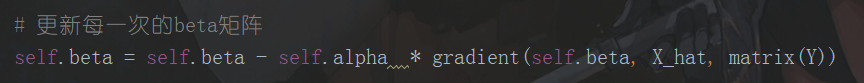
\includegraphics[scale=0.5]{try.png}\\
	
	这种情况对alpha的精度要求比较高,需要更多的loop才能获得同等的结果(70\%左右),并且观察cost\_function的difference的时候我发现波动比较大,常常有正值;
	
	并且这种方法需要比较多的loop才能获得相对准确的结果;因此我还是使用之前平均值的用于梯度的更新
	
	\item 观察到这次的数据数量级相近,因此不对数据进行归一化处理
\end{itemize}

\end{enumerate}
    
\end{solution}




%\begin{problem}[ML problem 4]

%\end{problem}
%\begin{solution}
   
%\end{solution}





%\begin{problem}[ML problem 5]

	%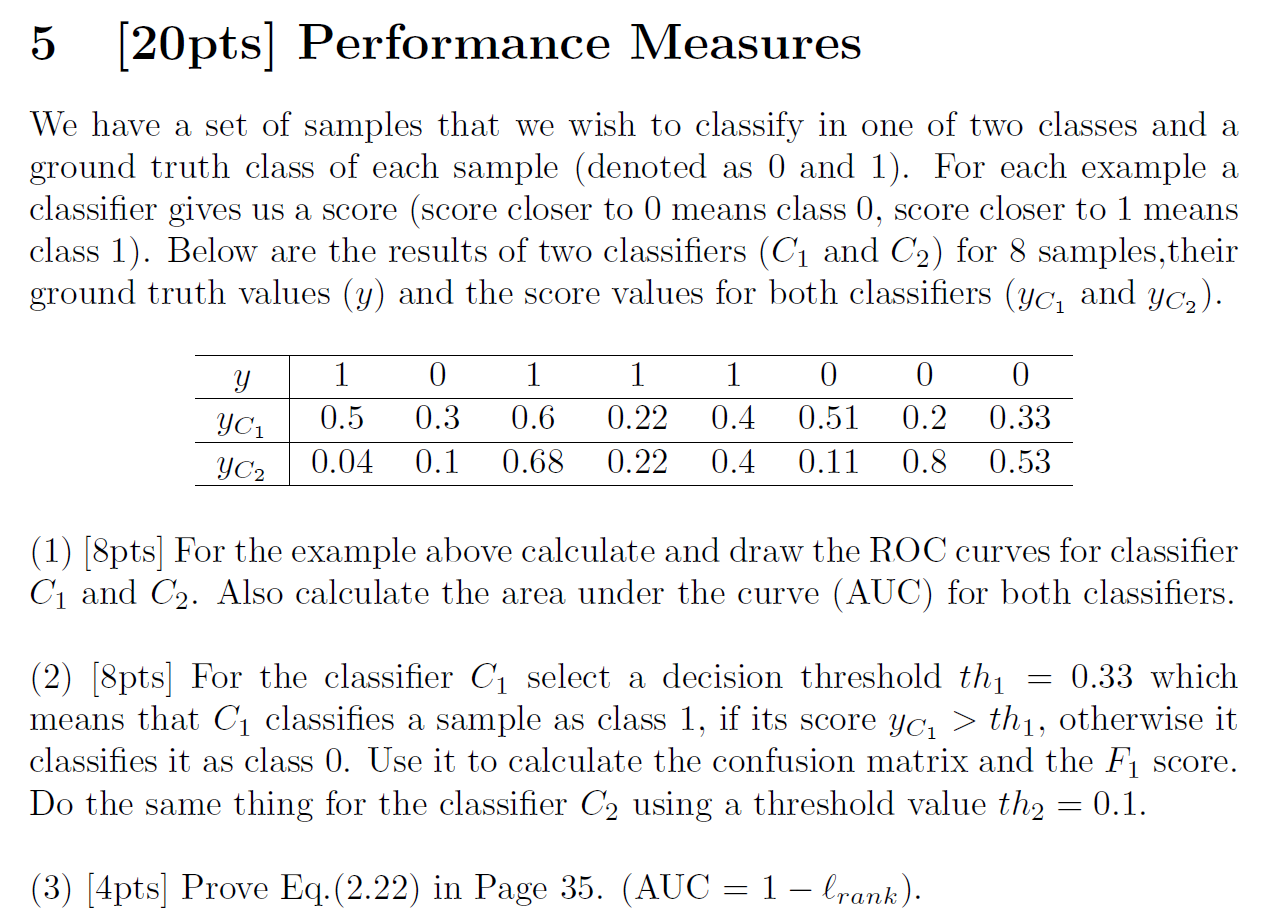
\includegraphics[scale=0.3]{5-p.png}

%\end{problem}
%\newpage
%\begin{solution}
   
%\end{solution}





%\begin{problem}[ML problem 6]
	
%\end{problem}
%\begin{solution}
    
%\end{solution}
%%%%%%%%%%%%%%%%%%%%%%%%%%%%%%%%%%%%%%%%%%%%%%%%%%%%%%%%%%%%%%%%
%                      Correction START!                       %
%%%%%%%%%%%%%%%%%%%%%%%%%%%%%%%%%%%%%%%%%%%%%%%%%%%%%%%%%%%%%%%%
%\begincorrection
%%%%%%%%%%%%%%%%%%%%
%\begin{problem}[]

%\end{problem}

%\begin{cause}
%
%\end{cause}

%\begin{revision}

%\end{revision}
%%%%%%%%%%%%%%%%%%%%
%\newpage
%%%%%%%%%%%%%%%%%%%%





%%%%%%%%%%%%%%%%%%%%%%%%%%%%%%%%%%%%%%%%%%%%%%%%%%%%%%%%%%%%%%%%
%                       Feedback START!                        %
%%%%%%%%%%%%%%%%%%%%%%%%%%%%%%%%%%%%%%%%%%%%%%%%%%%%%%%%%%%%%%%%
%\beginfb
%\begin{itemize}
%
%\end{itemize}





%%%%%%%%%%%%%%%%%%%%%%%%%%%%%%%%%%%%%%%%%%%%%%%%%%%%%%%%%%%%%%%%
%                        Homework END!                         %
%%%%%%%%%%%%%%%%%%%%%%%%%%%%%%%%%%%%%%%%%%%%%%%%%%%%%%%%%%%%%%%%
\end{document}
